\documentclass[8pt]{beamer} % default aspect ratio is 4:3
\usepackage{hyperref}
\usepackage{fontspec}
\usepackage[T1]{fontenc}
\setsansfont{Times New Roman}
\usefonttheme[onlymath]{serif}
% other packages
\usepackage{latexsym,amsmath,xcolor,multicol,booktabs,calligra}
\usepackage{graphicx,pstricks,listings,stackengine}
\usepackage{subcaption}

\author{Aryan Ahadinia / Ramtin Moslemi}
\title{Data Augmentation Can Improve Robustness}
\subtitle{A Paper Presentation \textit{for} Security and Privacy in Machine Learning}
\institute{Department of Computer Engineering, Sharif University of Technology}
\date{May 14, 2024}
\usepackage{spml}

% defs
\def\cmd#1{\texttt{\color{red}\footnotesize $\backslash$#1}}
\def\env#1{\texttt{\color{blue}\footnotesize #1}}
\definecolor{deepblue}{rgb}{0,0,0.5}
\definecolor{deepred}{RGB}{153,0,0}
\definecolor{deepgreen}{rgb}{0,0.5,0}
\definecolor{halfgray}{gray}{0.55}


\begin{document}

\begin{frame}
    \begin{figure}[htpb]
        \begin{center}
            
\includegraphics[keepaspectratio, scale=0.025]{pic/sut-logo.png}
        \end{center}
    \end{figure}
    \titlepage
    \vspace*{-0.6cm}
\end{frame}

\begin{frame}{A Paper of 35\textsuperscript{th} Conference on Neural Information Processing Systems}
    \begin{figure}
        \centering
        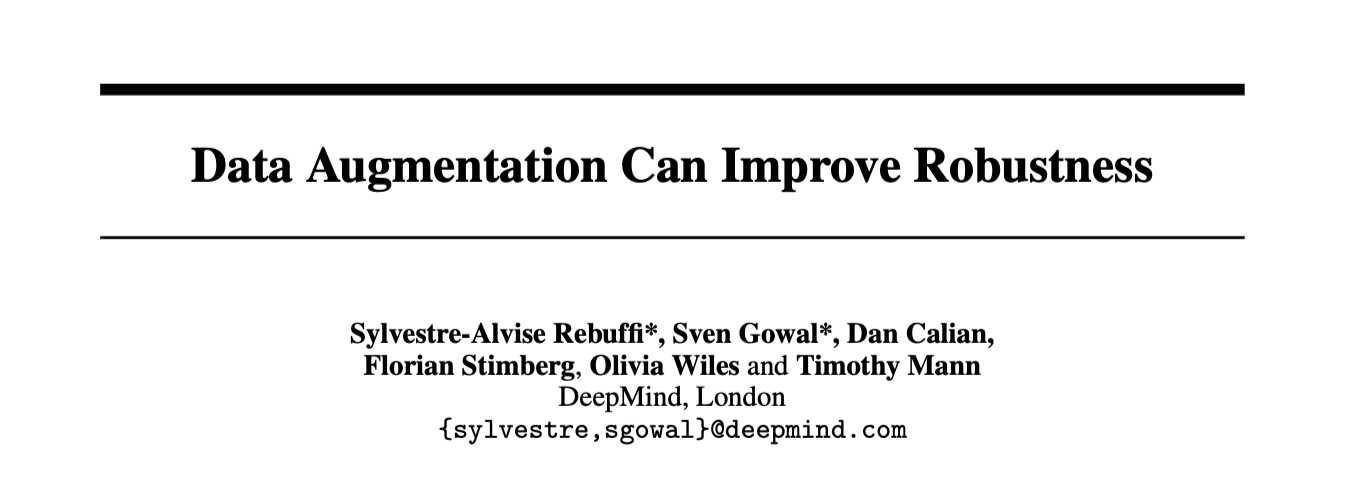
\includegraphics[width=\linewidth]{pic/Title.png}
        \label{fig:title}
    \end{figure}
\end{frame}

\begin{frame}{Today's Agenda}
    \tableofcontents[sectionstyle=show,
    subsectionstyle=show/shaded/hide,
    subsubsectionstyle=show/shaded/hide]
\end{frame}

\section{Introduction}

\begin{frame}{Abstract}
    \begin{itemize}
    % [<+-| alert@+>] % stepwise alerts
        \item Adversarial training suffers from \emph{robust over-fitting}.
        \item This paper focuses on reducing robust over-fitting by using \emph{data augmentation}.
        \item Contrary to previous findings, when combined with model weight averaging, data augmentation can significantly boost robust accuracy. 
    \end{itemize}
\end{frame}

\begin{frame}{Adversarial Examples}
    \begin{itemize}[<+-| alert@+>] % stepwise alerts
        \item Addition of imperceptible deviations to the input, called adversarial perturbations, can cause neural networks to make incorrect predictions with high confidence.
        \item The art of crafting increasingly sophisticated adversarial examples has received a lot of attention.
        \item Goodfellow et al. proposed the \href{https://arxiv.org/abs/1412.6572}{FGSM} which generates adversarial examples with a single normalized gradient step. 
        \item It was followed by \href{https://arxiv.org/pdf/1705.07204}{R+FGSM}, which adds a randomization step,
        \item and the \href{https://arxiv.org/abs/1607.02533}{BIM}, which takes multiple smaller gradient steps.
    \end{itemize}
\end{frame}

\begin{frame}{Adversarial Training}
    \begin{itemize}[<+-| alert@+>] % stepwise alerts
        \item Adversarial training as proposed by Madry et al. is so effective that it is the de facto standard for training adversarially robust neural networks.
        \item The adversarial training procedure feeds adversarially perturbed examples back into the training data by formulating a saddle point problem to find model parameters $\mathbf{\theta}$ that minimize the adversarial risk:
            $$\arg \min_\mathbf{\theta} \mathbb{E}_{(\mathbf{x},y)\sim \mathcal{D}}\left[\max_{\mathbf{\delta} \in \mathbb{S}} l(f(\mathbf{x}+\mathbf{\delta} ; \mathbf{\theta}), y)\right]$$
        \item To solve the inner optimization problem, we can use \href{https://arxiv.org/pdf/1706.06083}{PGD}, to replace the non-differentiable 0-1 loss $l$ with the cross-entropy loss $l_\text{ce}$ and compute an adversarial perturbation $\hat{\mathbf{\delta}}=\mathbf{\delta}^{(K)}$ in $K$ gradient ascent steps of size $\alpha$ as:
            $$\mathbf{\delta}^{(k+1)} \leftarrow \text{proj}_{\mathbb{S}}\left(\mathbf{\delta}^{(k)} + \alpha ~\text{sign}\left(\nabla_{\mathbf{\delta}^{(k)}}l_{\text{ce}}(f(\mathbf{x}+\mathbf{\delta}^{(k)};\mathbf{\theta}),y)\right)\right)$$
        \item It has been augmented in different ways – with changes in the attack procedure (e.g., by incorporating momentum), loss function (e.g., logit pairing) or model architecture (e.g., feature denoising).
        \item Adversarial training suffers from a phenomenon known as \emph{robust overfitting}.
    \end{itemize}
\end{frame}

\begin{frame}{Data Augmentation}
    \begin{itemize}[<+-| alert@+>] % stepwise alerts
        \item Data augmentation improves the generalization of standard (non-robust) training. 
        \item For image classification tasks, random flips, rotations and crops are commonly used. 
        \item There are more sophisticated techniques: 
            \begin{itemize}
                \item \textit{Cutout} which produces random occlusions
                \item \textit{CutMix} which replaces parts of an image with another
                \item \textit{MixUp} which linearly interpolates between two images
            \end{itemize}
        \begin{figure}
            \centering
            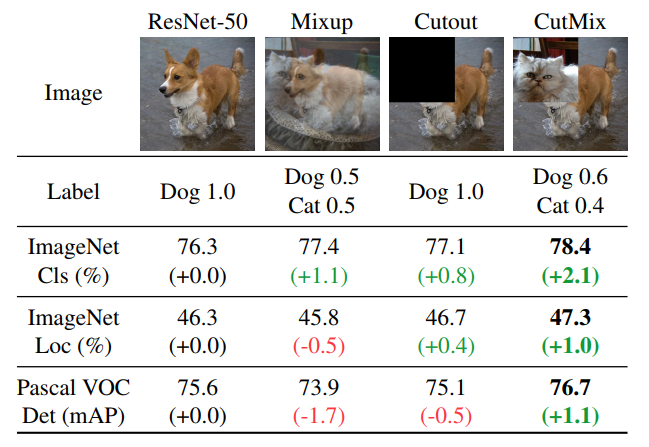
\includegraphics[width=0.5\linewidth]{pic/cutmix.png}
            % \caption{Caption}
            \label{fig:cutmix}
        \end{figure}
        \item Surprisingly they remain ineffective when training adversarially robust networks. 
        \item In this work, we revisit these common augmentation techniques.
    \end{itemize}
\end{frame}



\section{Preliminaries}

\begin{frame}{Preliminary Experiment}
    \begin{itemize}
        \item To study this issue, we begin with a preliminary experiment to test harmful queries for LLMs covering 30 languages, ranging from high-resource to low-resource.
        \item \textbf{Dataset \& Language}: We construct a curated dataset by gathering 15 harmful English prompts from the GPT-4 report. These intentionally crafted samples are designed to bypass safety mechanisms and have the potential to trigger the generation of harmful content in LLMs. We evaluate a diverse set of languages, from widely spoken to lesser-known ones.
        \item \textbf{Model \& Evaluation}: We evaluate ChatGPT (GPT-3.5-turbo-0613) for its significant impact and strong multilingual capabilities, using a temperature of 0 for consistency. The outputs are classified as:
        \begin{itemize}
            \item \textbf{Safe}: free of harmful content or decline to answer unsafe questions
            \item \textbf{Unsafe}: contain harmful content or directly address unsafe queries
            \item \textbf{Invalid}: unrelated or unnatural, irrelevant or incoherent answers for non-English queries 
        \end{itemize}
    \item Our main focus is identifying and reporting the unsafe rate, and the percentage of unsafe responses among all generated by the target LLMs.
    \end{itemize}
\end{frame}

\begin{frame}{Language Selection}
    \begin{itemize}
        \item We determine the resource levels for each language by utilizing the data ratio from the CommonCrawl corpus, which is the primary dataset for most LLMs’ pre-training. 
        \item A language is categorized as:
        \begin{itemize}
            \item \textbf{HRL}: high-resource if its data ratio exceeds 1\%
            \item \textbf{MRL}: medium-resource if its data ratio falls between 0.1\% and 1\%
            \item \textbf{LRL}: low-resource if its data ratio is below 0.1\%
        \end{itemize}
    \end{itemize}
    \begin{figure}
            \centering
            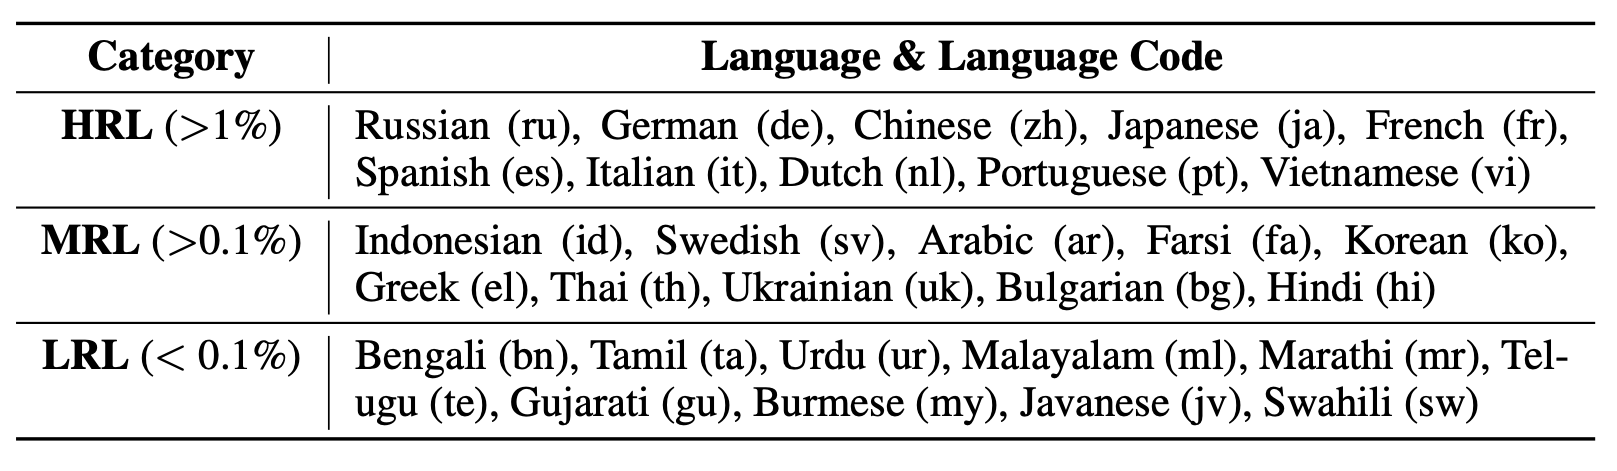
\includegraphics[width=\linewidth]{pic/language selection.png}
            \caption{Language selection in preliminary experiments.}
            \label{fig:language_selection}
    \end{figure}
\end{frame}

\begin{frame}{Preliminary Results}
    \begin{itemize}
        \item LLMs can effectively defend against harmful queries in high-resource languages, their performance declines with decreasing resource availability.
        \item This reveals a correlation between decreased language resources and an increased rate of unsafe outputs, indicating potential risks for low-resource language speakers.
        \item These findings also show the potential of multilingualism as a jailbreak method.
    \end{itemize}
    \begin{figure}
            \centering
            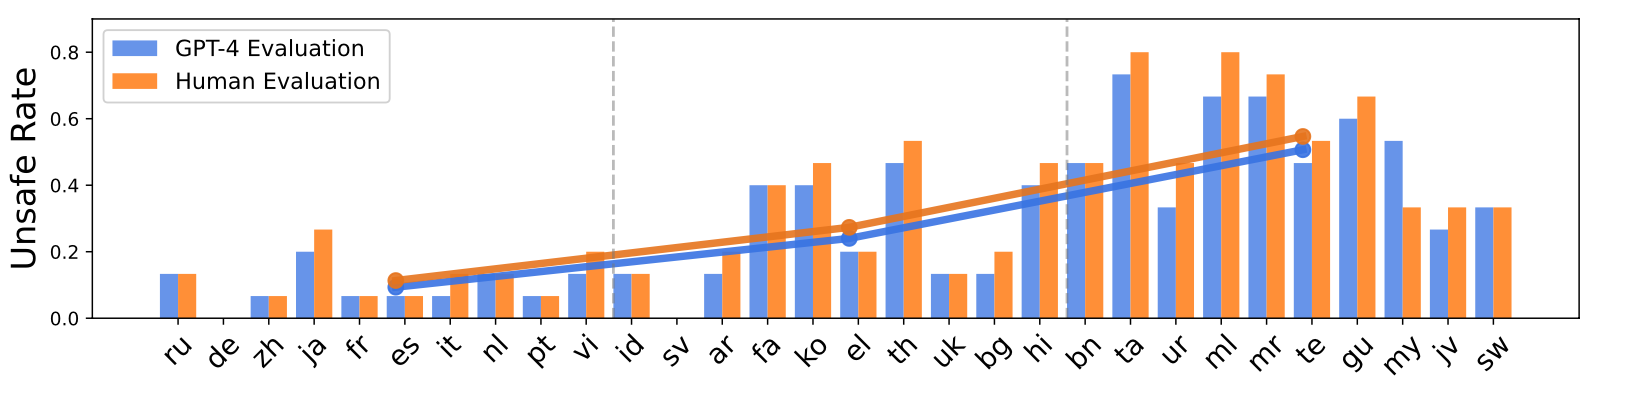
\includegraphics[width=\linewidth]{pic/Prelim Results.png}
            \caption{Preliminary results on curated dataset. The line plot shows averaged results for three language categories, indicating an increasing unsafe rate as language availability decreases.}
            \label{fig:prelim_results}
        \end{figure}
\end{frame}

\begin{frame}{Risk Scenarios}
    \begin{itemize}
        \item \textbf{Unintentional}: This highlights the heightened risk faced by speakers of low-resource languages regarding exposure to harmful content. Due to the limitations imposed by resource availability, LLMs may struggle to effectively filter or prevent the generation of unsafe responses. This poses a significant challenge for individuals relying on these models, as they may unknowingly encounter harmful or biased information.
        \item \textbf{Intentional}: Malicious actors may take advantage of the vulnerabilities in these models to intentionally map their harmful prompts into low-resource languages, through translation services such as Google Translate. Additionally, they may even combine these prompts with malicious instructions obtained from online sources, thereby amplifying the potential for further attacks.
    \end{itemize}
\end{frame}

\section{Data Augmentation Can Improve Robustness}

\begin{frame}{Contributions}
    \begin{itemize}[<+-| alert@+>] % stepwise alerts
        \item Demonstrate data augmentation techniques such as \textit{Cutout}, \textit{CutMix} and \textit{MixUp} can improve robustness when paired with WA.
        \item To the contrary of \href{https://arxiv.org/pdf/2010.03593}{Gowal et al.}, Rice et al., Wu et al. we are able to use any of these three aforementioned techniques to obtain new \emph{state-of-the-art robust accuracies}. 
        \begin{figure}
            \begin{minipage}[c]{0.45\linewidth}
                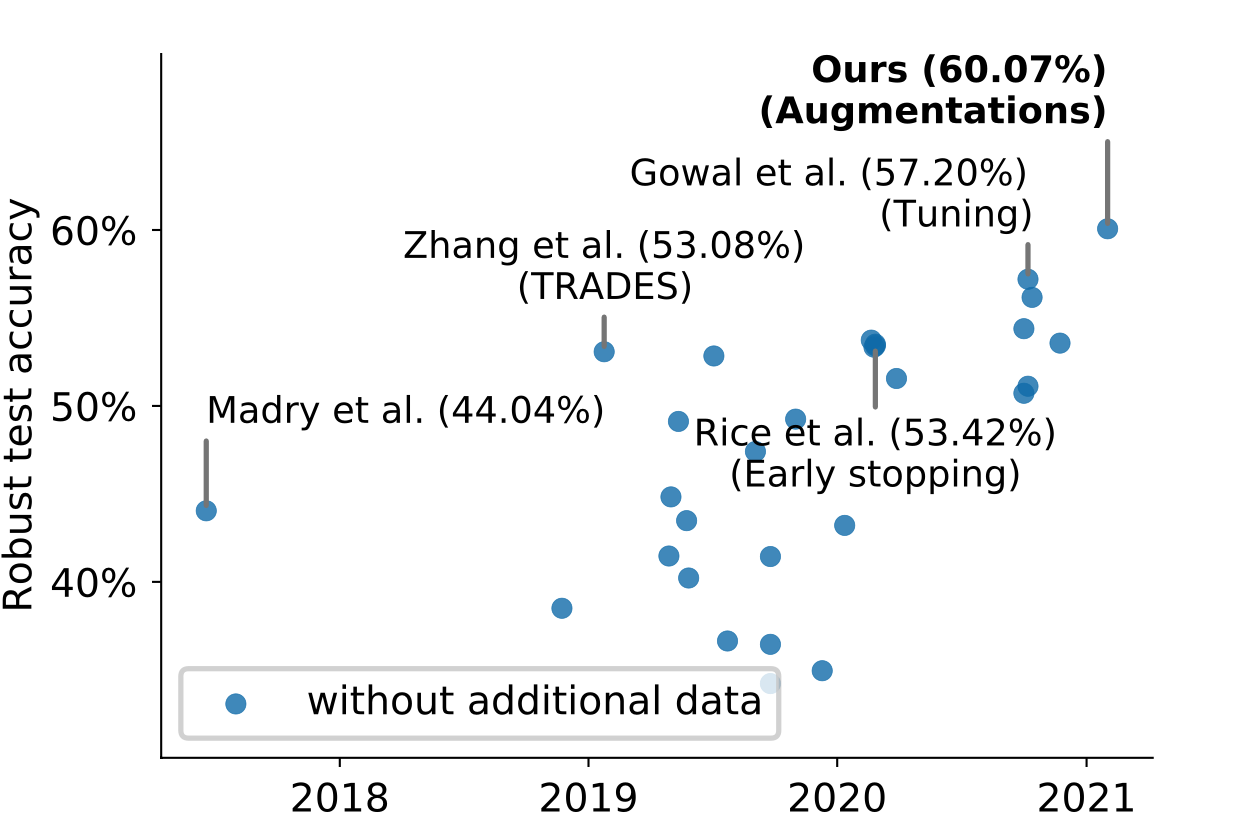
\includegraphics[width=\linewidth]{pic/sota.png}
            \end{minipage}
            \begin{minipage}[c]{0.45\textwidth}
                \caption{Robust accuracy of various models submitted to RobustBench against AUTOATTACK on CIFAR-10 with $\ell_\infty$ perturbations of size $8/255$ displayed in publication order. Our method builds on \href{https://arxiv.org/pdf/2010.03593}{Gowal et al.} and explores how augmented data can be used to improve robust accuracy by $+2.87\%$ without using any additional external data.} \label{fig:sota}
            \end{minipage}
        \end{figure}
        \item Show that approach generalizes across architectures, datasets and threat models.
        \item Investigate the trade-off between robust overfitting and underfitting.
        % to explain why \textit{MixUp} performs worse than spatial composition techniques.
        \item Provide empirical evidence that WA exploits data augmentation by ensembling snapshots.
    \end{itemize}
\end{frame}

\begin{frame}{Hypothesis}
    \begin{itemize}[<+-| alert@+>] % stepwise alerts
        \item As WA results in flatter, wider solutions compared to the steep decrease in robust accuracy observed for SGD, it is natural to ask ourselves whether WA remains useful in cases that do not exhibit robust overfitting.
        \item We notice that the robust performance in this setting is not only preserved but even boosted when using WA. 
        \item Hence, we formulate the hypothesis that: 
            \begin{quote}
                \emph{model weight averaging helps robustness to a greater extent when robust accuracy between model iterations can be maintained.}
            \end{quote}
        \item This hypothesis is also motivated by the observation that WA acts as a temporal ensemble – akin to Fast Geometric Ensembling by \href{https://arxiv.org/pdf/1802.10026}{Garipov et al.} who show that efficient ensembling can be obtained by aggregating multiple checkpoint parameters at different training times.
    \end{itemize}
\end{frame}

\begin{frame}{Limiting Robust Overfitting Without External Data}
    \begin{itemize}
        \item Rice et al. show that combining data augmentation methods such as \textit{Cutout} or \textit{MixUp} with early stopping does not improve robustness upon early stopping alone. 
        \item While, these methods do not improve upon the “best” robust accuracy, they reduce the extent of robust overfitting, thus resulting in a slower decrease in robust accuracy compared to classical adversarial training (which uses random crops and weight decay). 
        \begin{figure}
            \begin{minipage}[c]{0.6\linewidth}
                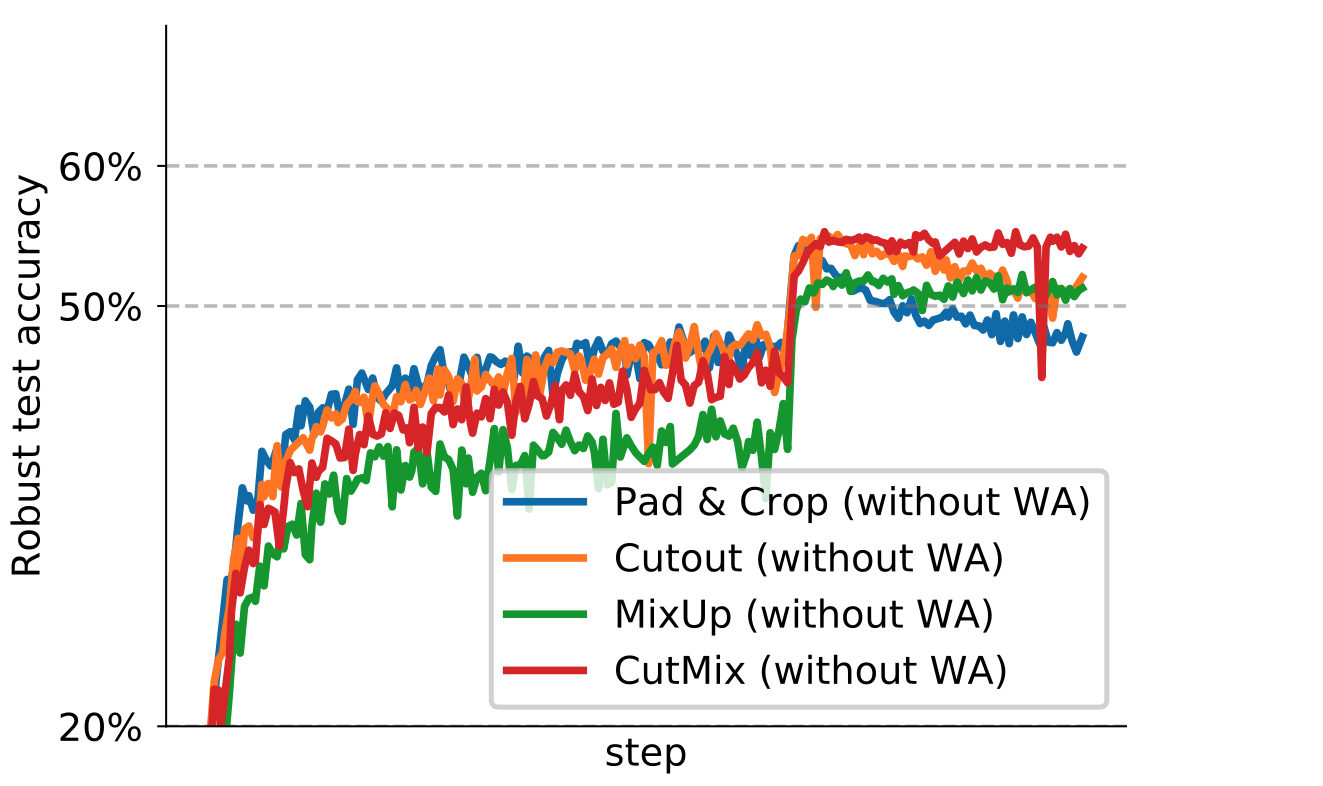
\includegraphics[height=.4\textheight]{pic/data_aug.png}
            \end{minipage}
            \begin{minipage}[c]{0.35\linewidth}
                \caption{Accuracy against $\epsilon_\infty = 8/255$ on CIFAR-10 without using model WA for different data augmentation schemes. The model is a WRN-28-10 and the panel shows the evolution of the robust accuracy as training progresses (against $PGD^{40}$). The jump in robust accuracy two-thirds through training is due to a drop in learning rate.}\label{fig:data_aug}
            \end{minipage}
        \end{figure}
    \end{itemize}
\end{frame}

\begin{frame}{Testing the Hypothesis}
    % \begin{itemize}
        % \item Since \textit{MixUp} preserves robust accuracy while \textit{Pad \& Crop} does not, this comparison can be used to evaluate the hypothesis that WA is more beneficial when the performance between model iterations is maintained.
        \begin{figure}
            \centering
            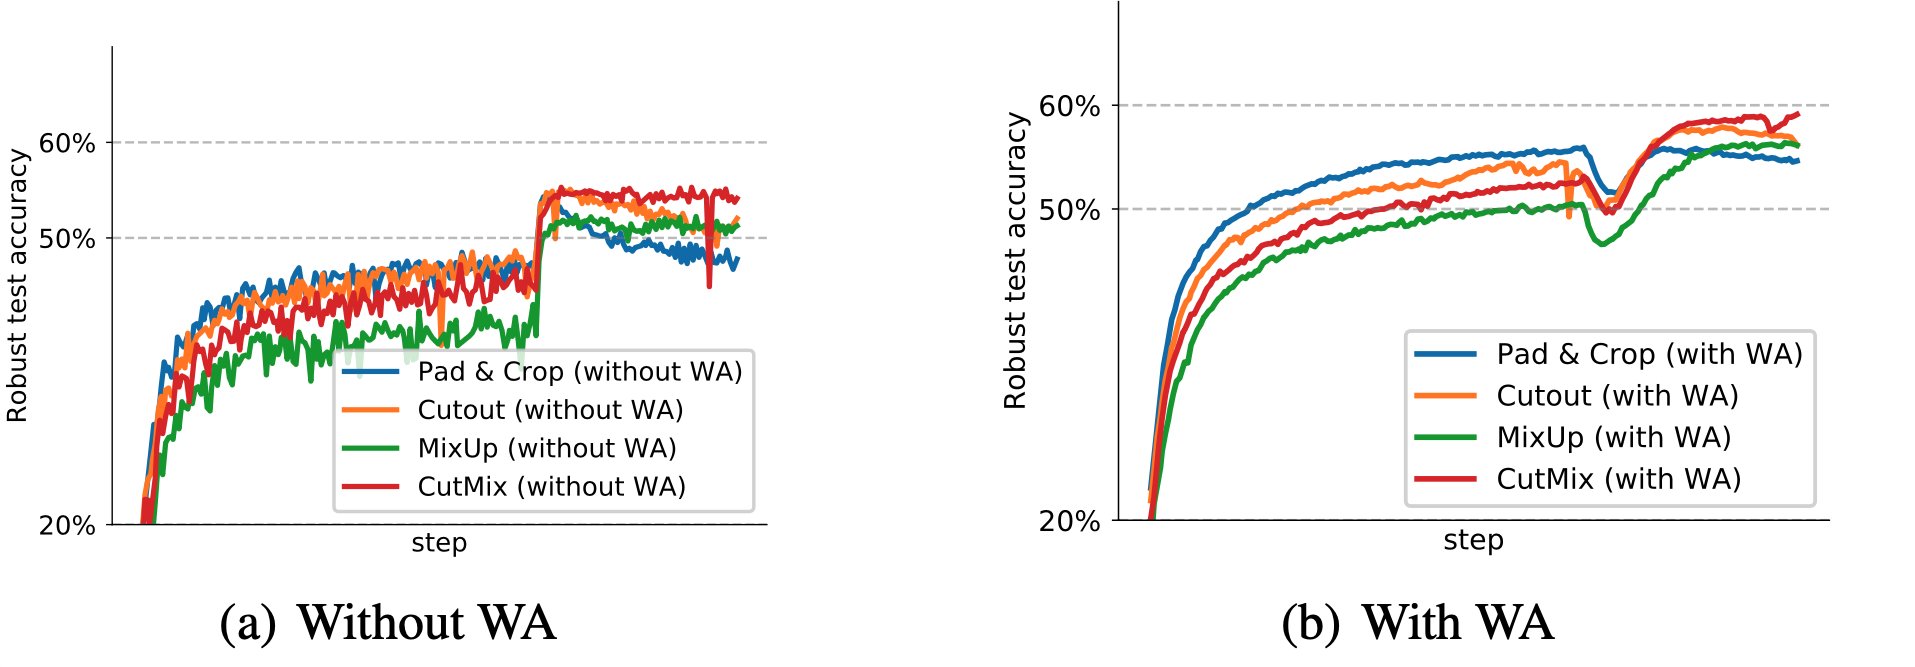
\includegraphics[height=.4\textheight]{pic/data_aug_wa.png}
            \caption{Accuracy against $\epsilon_\infty = 8/255$ on CIFAR-10 without using model weight averaging (WA) for different data augmentation schemes. The model is a WRN-28-10 and both panels show the evolution of the robust accuracy as training progresses (against $PGD^{40}$). The jump in robust accuracy two-thirds through training is due to a drop in learning rate. The accuracy drop just after the change of learning rate stems from averaging very different weights.}
            \label{fig:data_aug_wa}
        \end{figure}
    % \end{itemize}
\end{frame}

\begin{frame}{Experimental Setup}
    \begin{itemize}[<+-| alert@+>] % stepwise alerts
        \item \textbf{Architecture.} We use WRNs as our backbone network. Most of the experiments are conducted on a WRN-28-10 model which has a depth of 28, a width multiplier of 10 and contains 36M parameters. To evaluate the effect of data augmentations on wider and deeper networks, we also run several experiments using WRN-70-16, which contains 267M parameters.
        \item \textbf{Outer minimization.} We use TRADES optimized using SGD with Nesterov momentum and a global weight decay of $5 \times 10^{-4}$.
        \item \textbf{Inner minimization.} Adversarial examples are obtained by maximizing the Kullback-Leibler divergence between the predictions made on clean inputs and those made on adversarial inputs. 
        \item \textbf{Evaluation.} We train two (and only two) models for each hyperparameter setting, perform early stopping for each model on a separate validation set using $PGD^{40}$. Finally, we report the robust test accuracy against a mixture of AUTOATTACK and MULTITARGETED, which is denoted by AA+MT.
    \end{itemize}
\end{frame}

\section{Results and Conclusion}

\begin{frame}{Comparing Data Augmentations}
    \begin{itemize}
        \item WA is the most beneficial when robust overfitting is reduced.
    \item Spatial composition techniques which outperform blending techniques.
        \begin{figure}
            \centering
            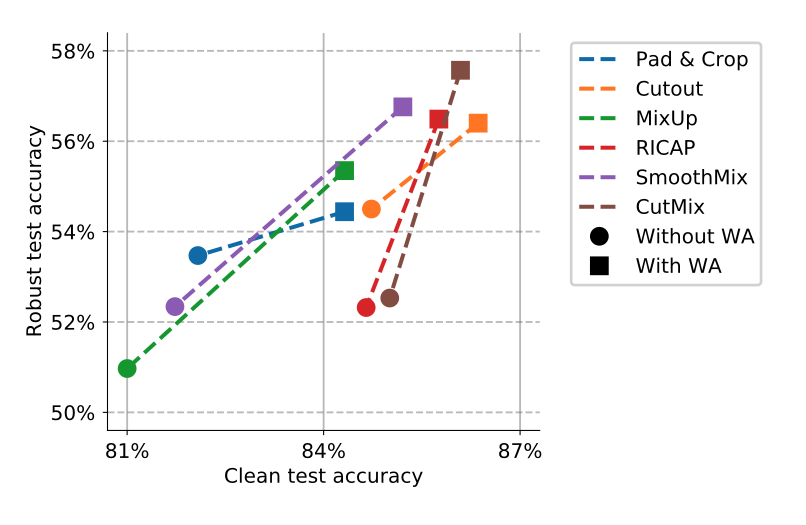
\includegraphics[height=.5\textheight]{pic/fig 4.png}
            \caption{Clean (without adversarial attacks) accuracy and robust accuracy (against AA+MT) for a WRN-28-10 trained against $\epsilon_\infty = 8/255$ on CIFAR-10 for different data augmentation techniques. The lines from circles to squares represent the performance change obtained when using WA.}
            \label{fig:fig4}
            \end{figure}
    \end{itemize}
\end{frame}

\begin{frame}{Blending Techniques}
    \begin{itemize}
        \item \textit{MixUp} samples the image mixing weight with a beta distribution $\text{Beta}(\alpha, \alpha)$
        \begin{itemize}
            \item tends to either produce images that are far from the original data distribution (when $\alpha$ is large)
            \item or too close to the original samples (when $\alpha$ is small)
        \end{itemize}
        \item Increasing $\alpha$ can lead to robust underfitting while an $\alpha$ too close to 0 would lead to robust overfitting.
        \begin{figure}
            \centering
            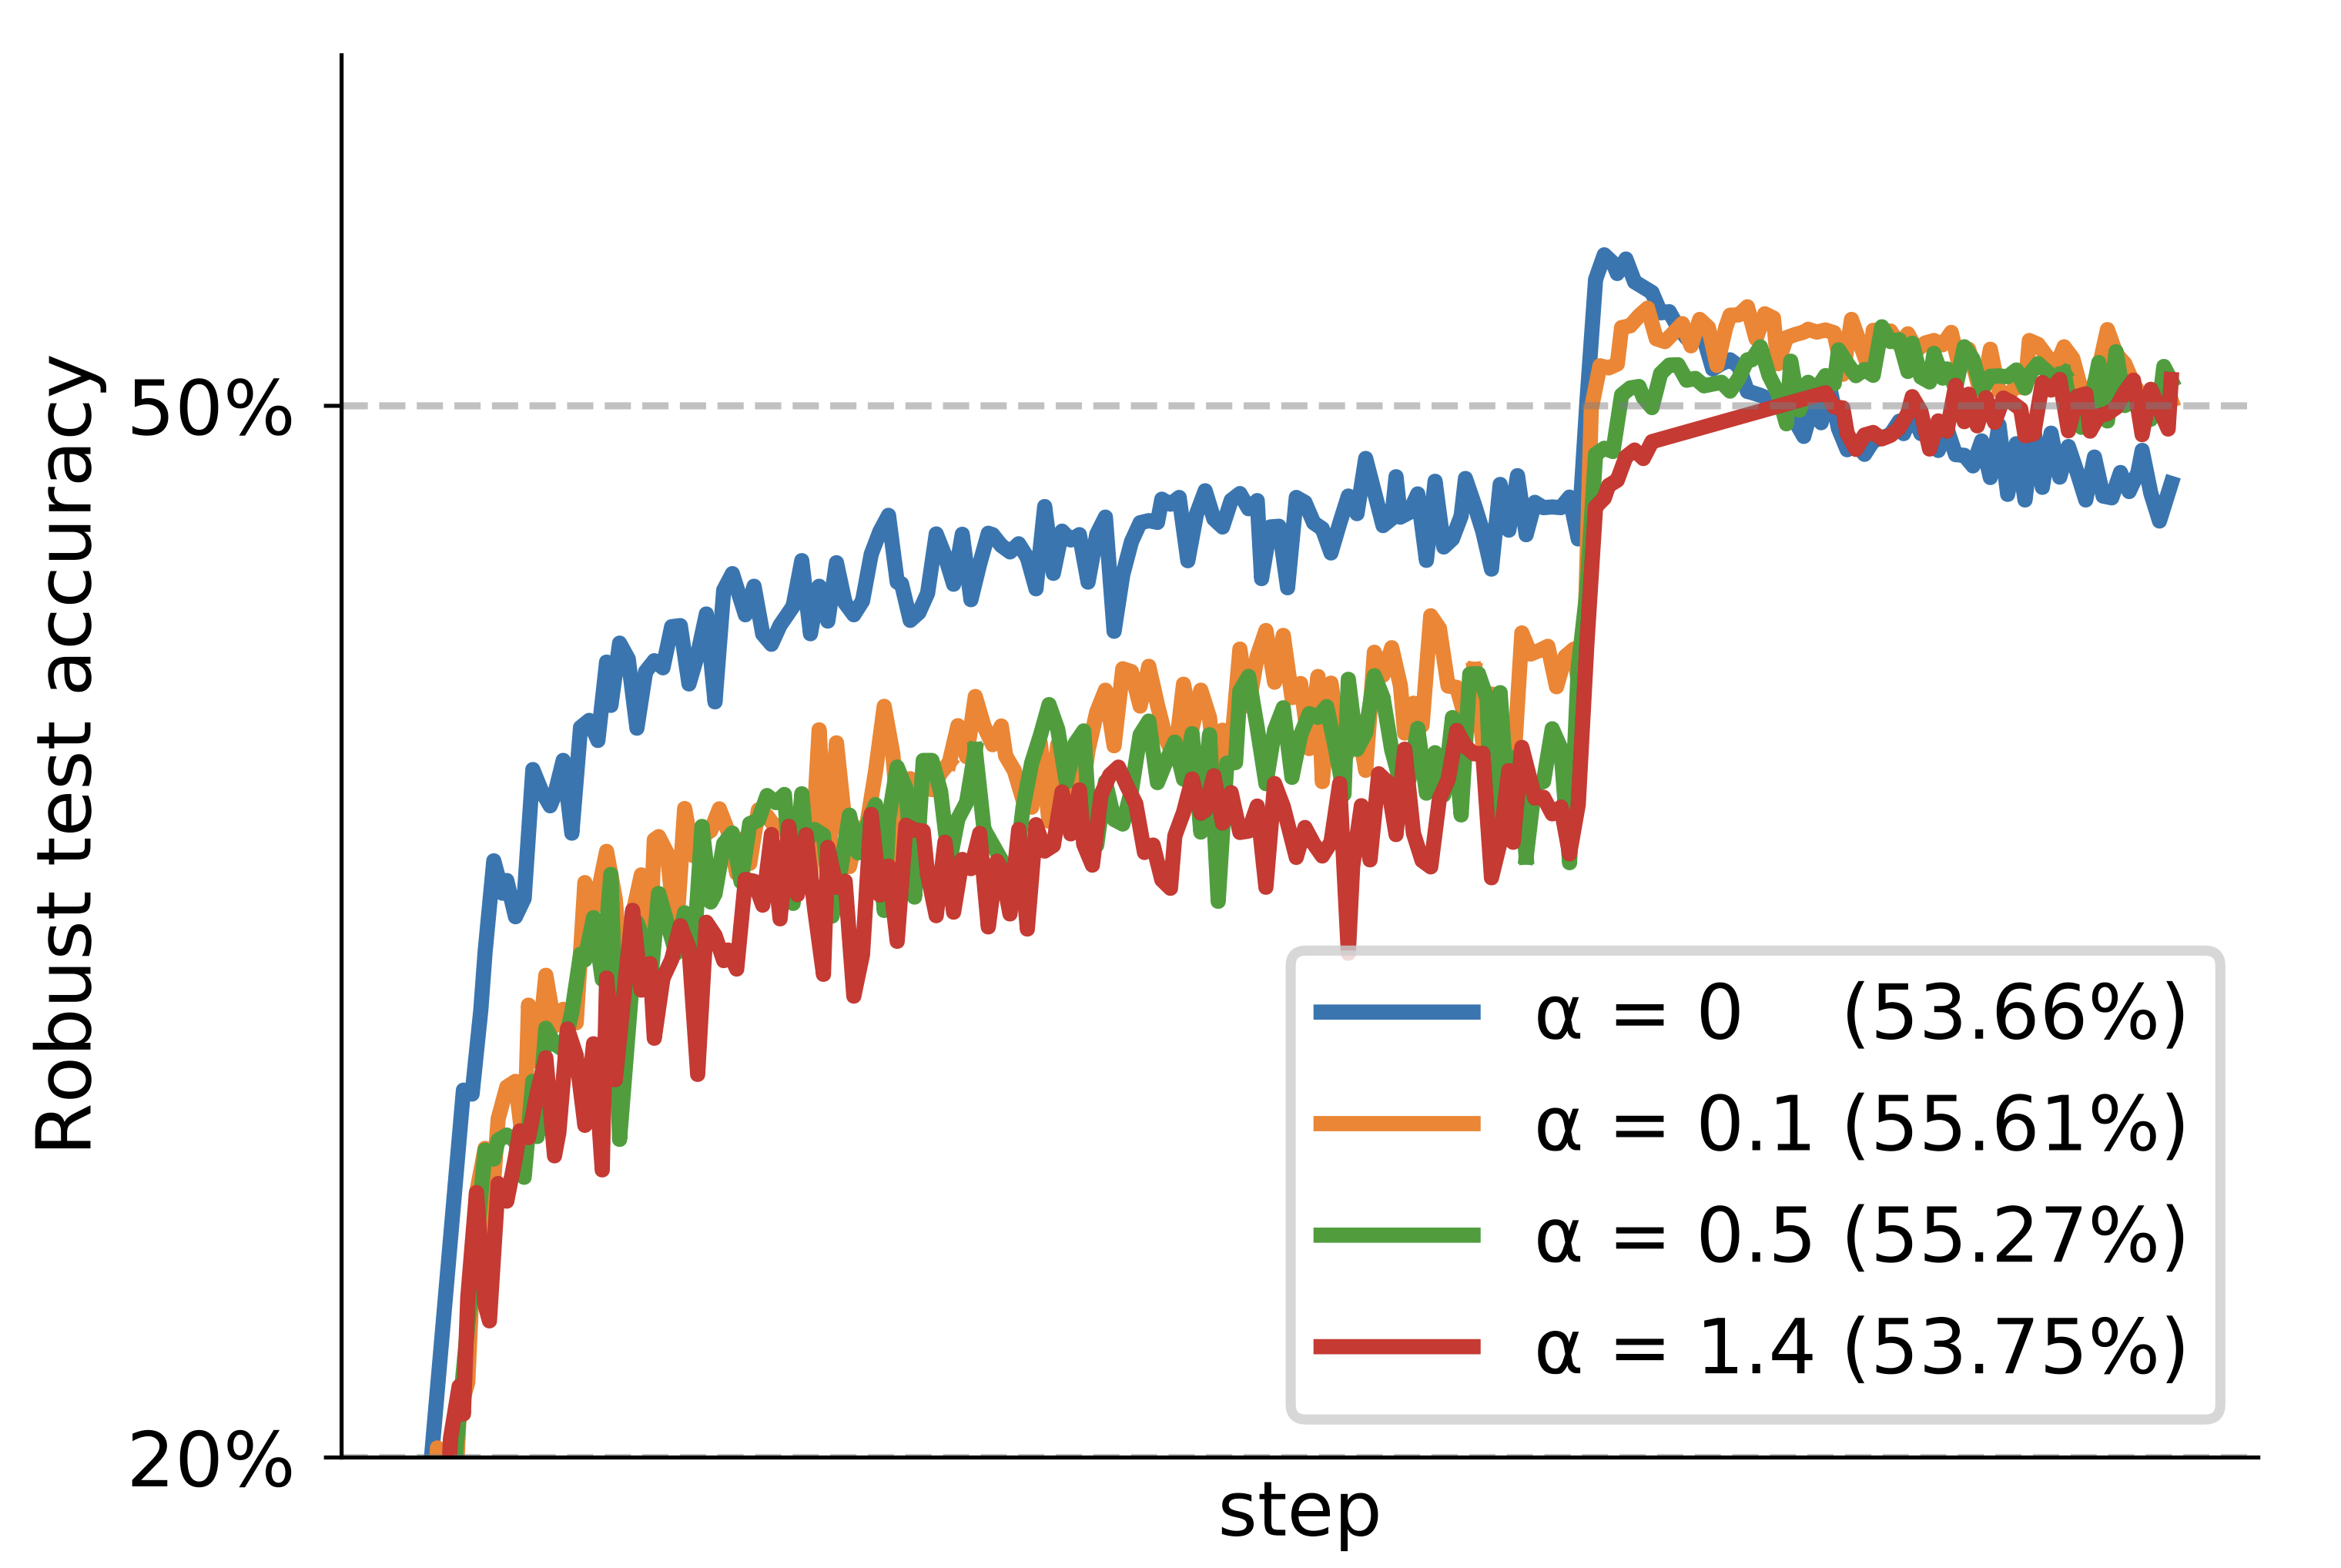
\includegraphics[height=0.4\textheight]{pic/mixup.png}
            \caption{The graph shows the robust test accuracy against $PGD^{40}$ with $\epsilon_\infty = 8/255$ on CIFAR-10 without using WA as we vary the mixing rate $\alpha$ of \textit{MixUp}. We report in the legend the robust accuracy (against AA+MT) after applying weight averaging to the corresponding runs.}
            \label{fig:fig5}
        \end{figure}
    \end{itemize}
\end{frame}

\begin{frame}{Spatial Composition Techniques}
\begin{itemize}
    \item \textit{Cutout} and \textit{CutMix} are most beneficial when using large window lengths.
    \item Low-level features tend to be destroyed by \textit{MixUp},
    \item whereas composition techniques locally maintain these low-level features. 
    \item Hence, we hypothesize augmentations designed for robustness need to preserve low-level features.
        \begin{figure}
            \centering
            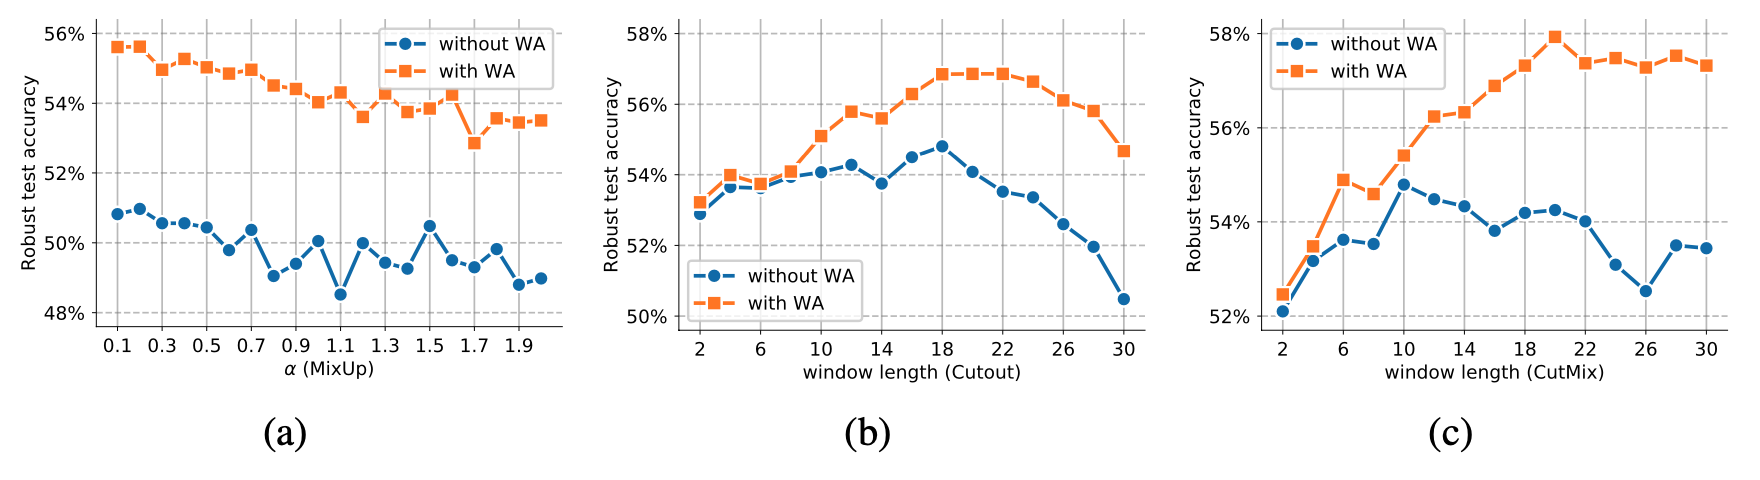
\includegraphics[height=.3\textheight]{pic/data_aug_res.png}
            \caption{Robust test accuracy against AA+MT with $\epsilon_\infty = 8/255$ on CIFAR-10 as we vary (a) the mixing rate α of MixUp, (b) the window length when using Cutout and (c) the window length when using CutMix. The model is a WRN-28-10 and we compare the settings without and with WA. 
            % As a reference when training only with Pad \& Crop, the same model with WA and without WA reaches $54.44\%$ and $53.66\%$ robust accuracy, respectively. Similarly, without any augmentation, the models with WA and without WA achieve $49.74\%$ and $42.27\%$, respectively.
            }
            \label{fig:data_aug_res}
        \end{figure}
    \end{itemize}
\end{frame}

\begin{frame}{Generalizing to other Architectures}
    \begin{figure}
        \centering
        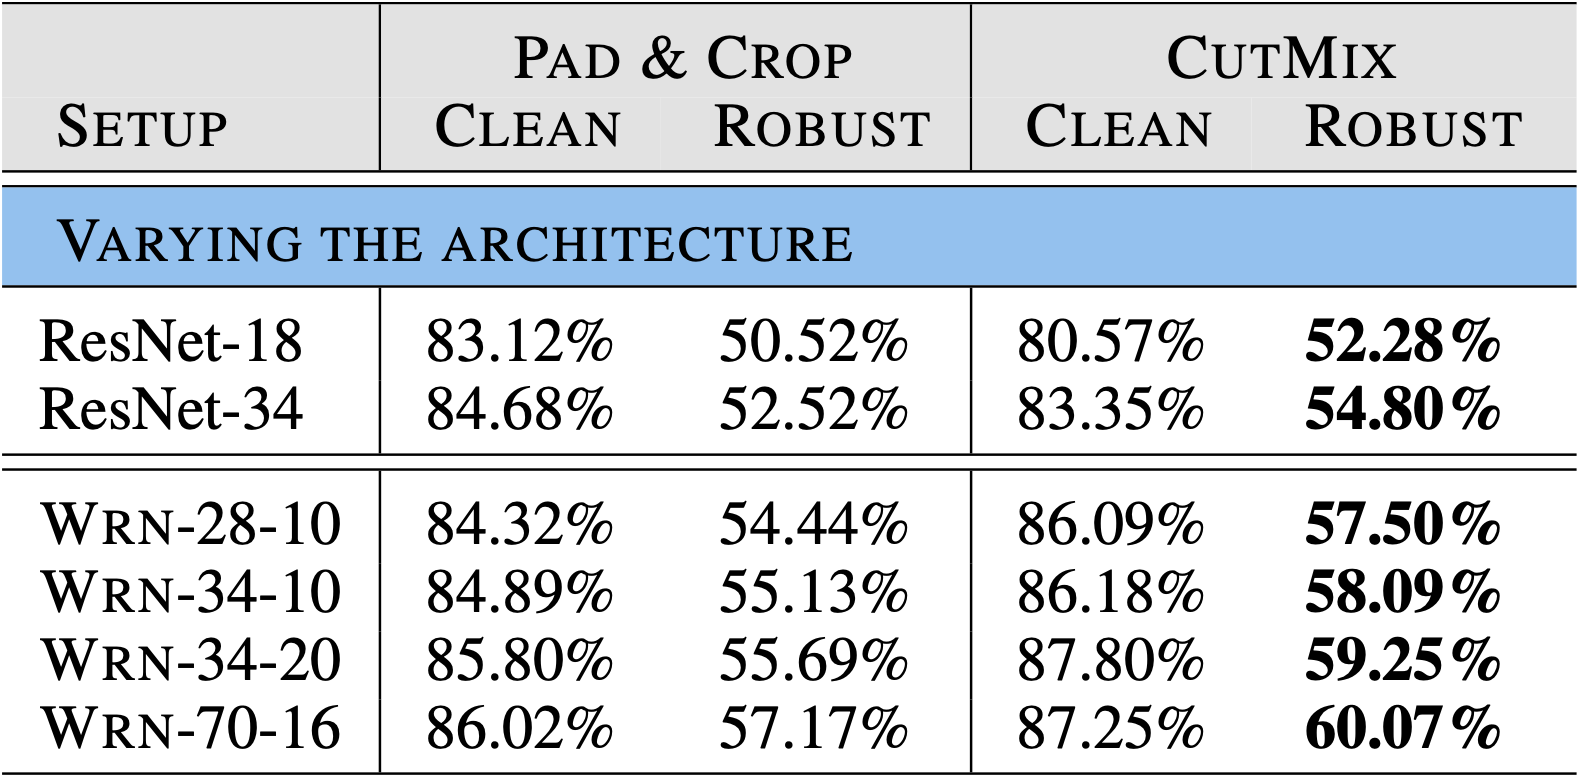
\includegraphics[width=\linewidth]{pic/Gen_Arch.png}
            \caption{Robust test accuracy (against AA+MT) against $\epsilon_\infty = 8/255$ on CIFAR-10 for different architectures. In all cases, we use weight averaging and we compare \textit{Pad \& Crop} and \textit{CutMix}.}
        \label{fig:gen_arch}
    \end{figure}
\end{frame}

\begin{frame}{Generalizing to other Threat Models}
    \begin{figure}
        \centering
            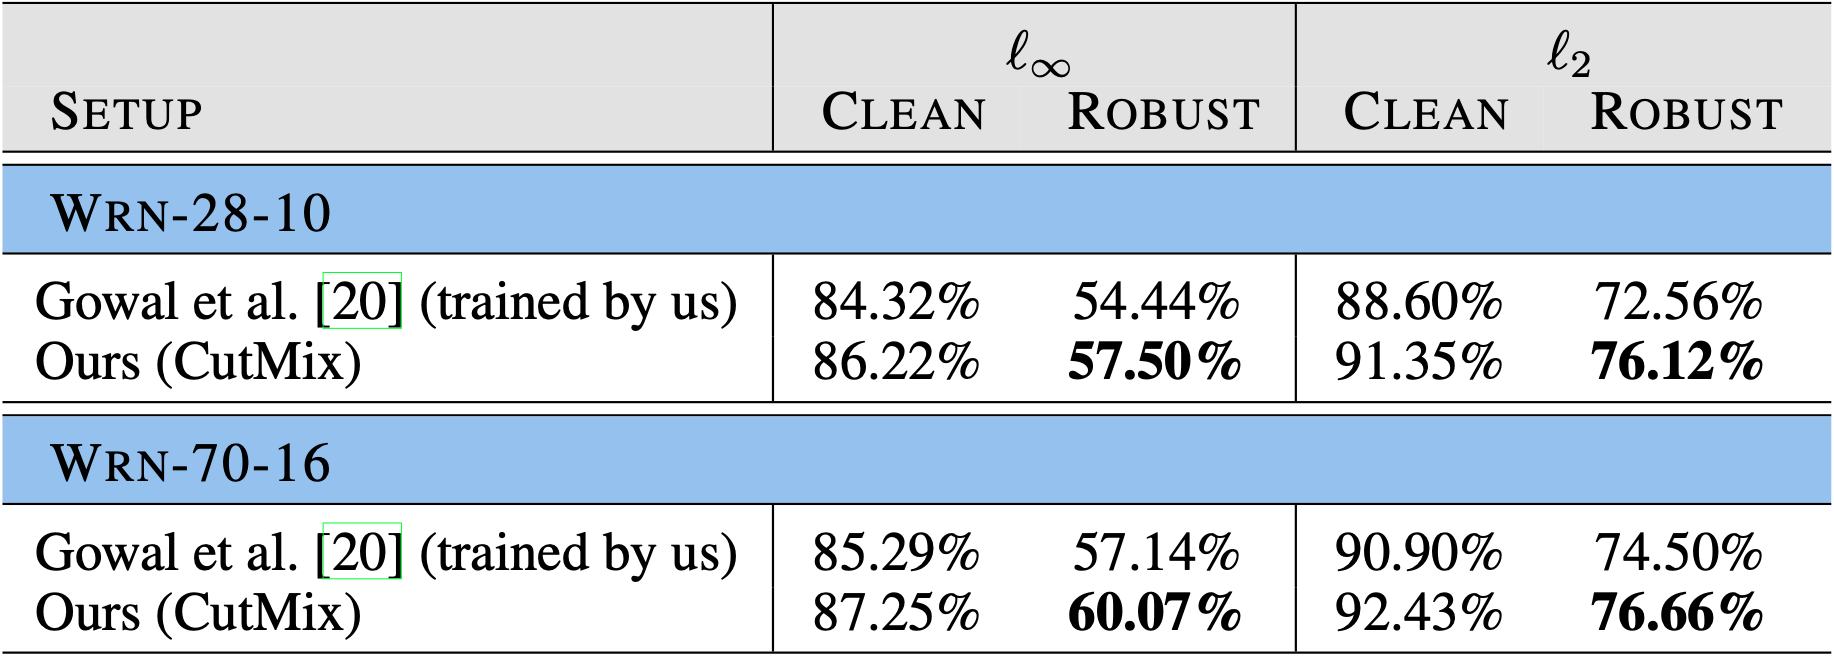
\includegraphics[width=\linewidth]{pic/Gen_Threat.png}
            \caption{Clean (with and without adversarial attacks) accuracy and robust accuracy (against AA+MT) on CIFAR-10 as we both test against $\epsilon_\infty = 8/255$ and $\epsilon_2 = 128/255$.}\label{fig:gen_threat}
    \end{figure}
\end{frame}

\begin{frame}{Generalizing to other Datasets}
    \begin{figure}
        \centering
        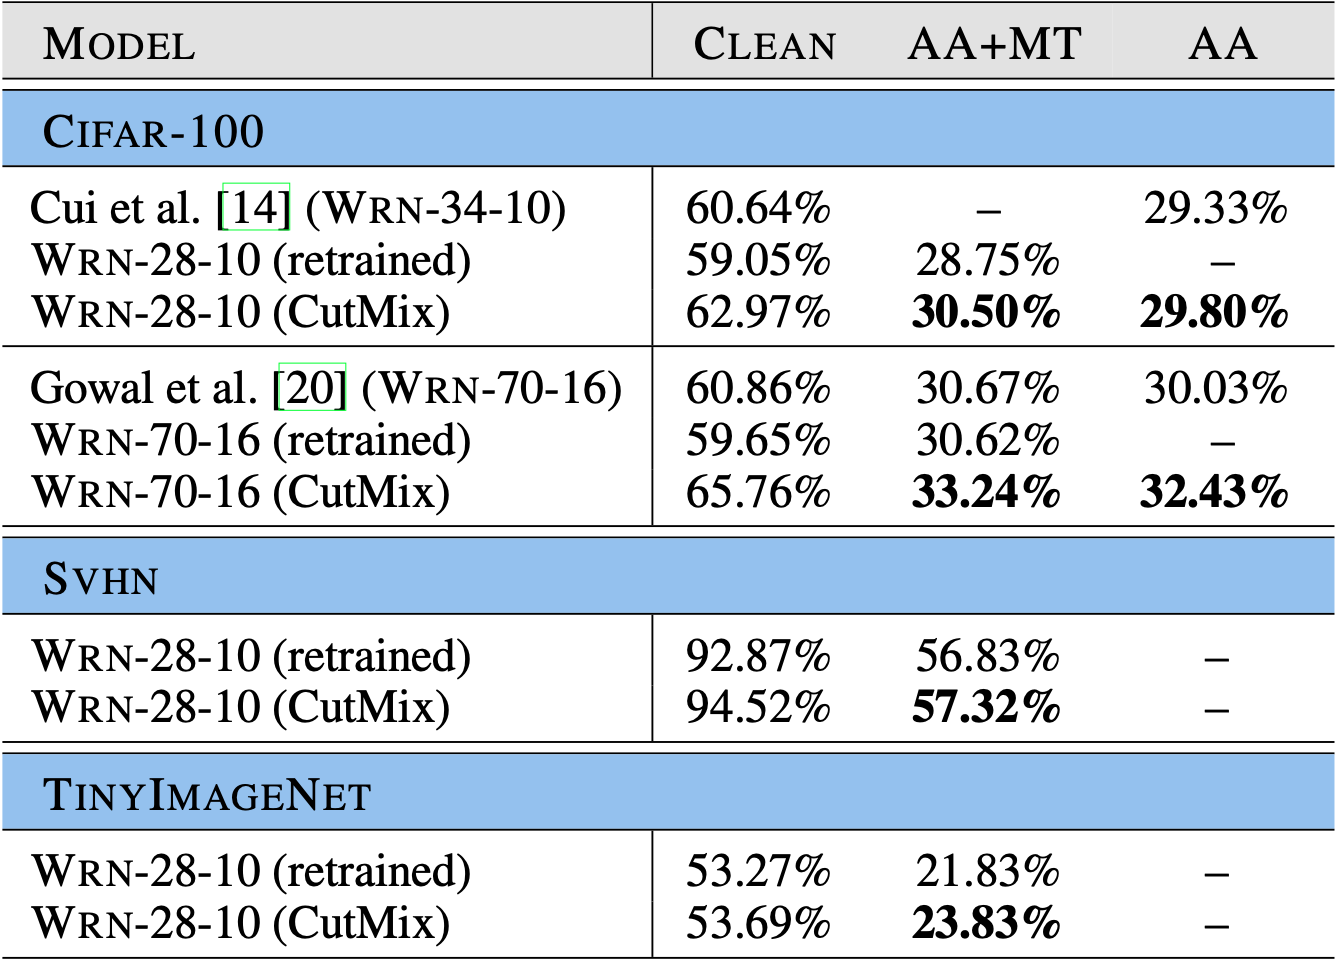
\includegraphics[width=0.7\linewidth]{pic/Gen_Data.png}
        \caption{Clean and robust accuracy (AA+MT and AutoAttack for select models) on CIFAR-100, SVHN and TINY-IMAGENET against $\epsilon_\infty = 8/255$ obtained by different models (with WA). The ’retrained’ indication means that the models have been retrained according to Gowal et al.’s methodology.}
        \label{fig:gen_data}
    \end{figure}
\end{frame}

\begin{frame}{Model Ensembling by Weight Averaging}
    Ensembling improves robustness by exploiting the diversity of equally performing models 
    \begin{figure}
        \centering
        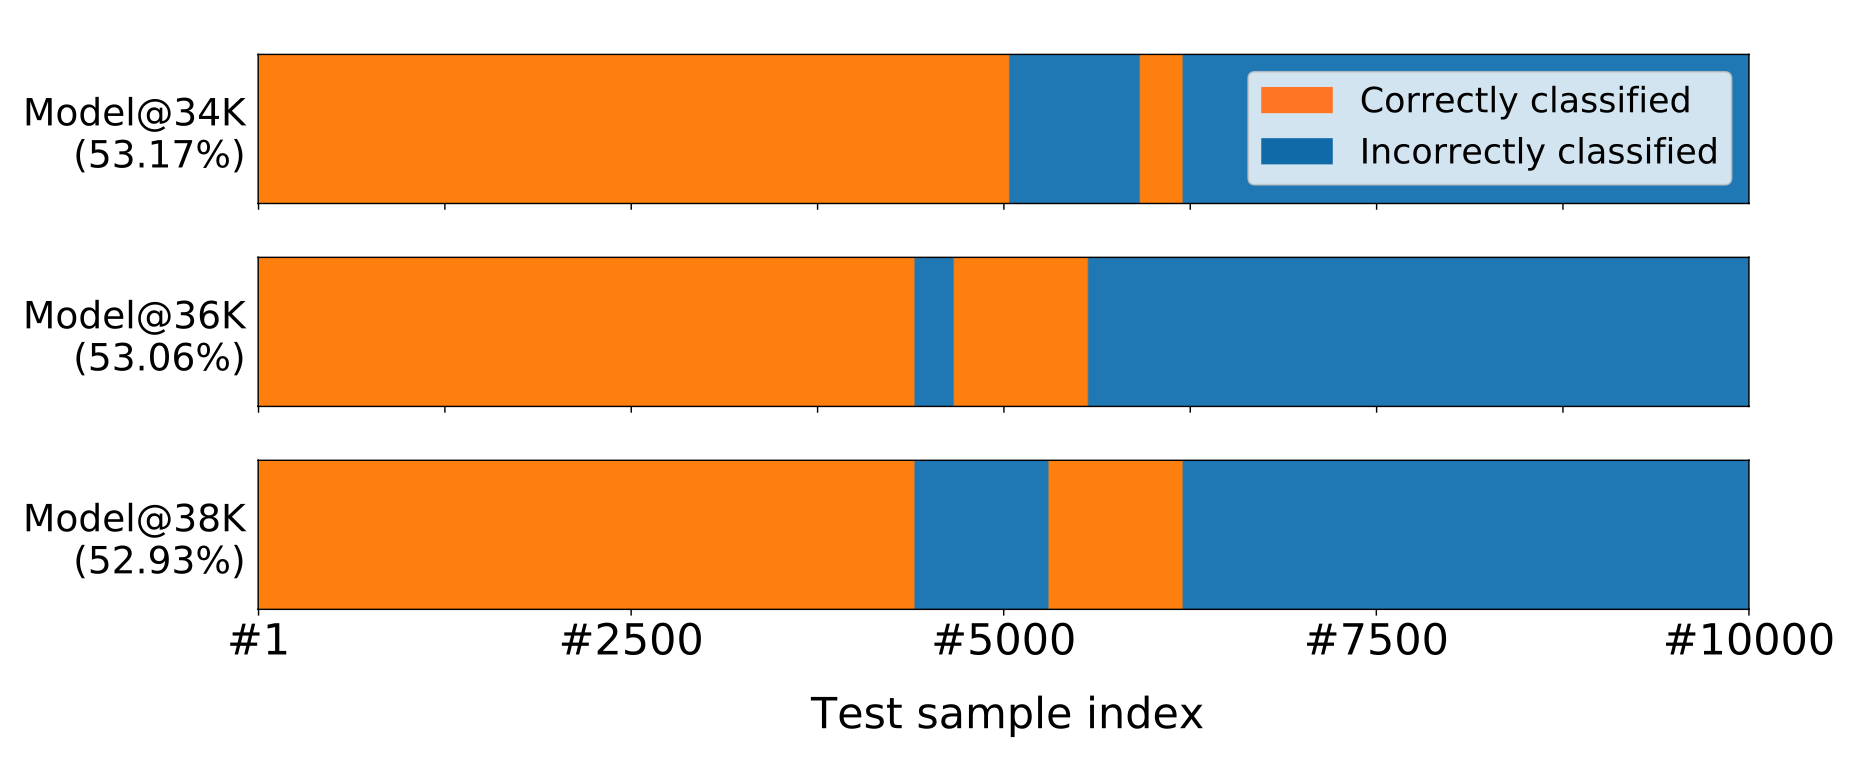
\includegraphics[width=\linewidth]{pic/fig 7.png}
        \caption{The bar plots show the outcome of each individual robust prediction for different snapshots of a same training run of a WRN-28-10 against $\epsilon_\infty = 8/255$ on CIFAR-10 without model weight averaging. The test sample indices have been re-ordered such as to show contiguous blocks. The plots show a significant variation in individual robust predictions across different snapshots while the total robust accuracy (i.e. the number in parenthesis) remains stable.}
        \label{fig:fig7}
    \end{figure}
\end{frame}

\begin{frame}{Limits of Exploiting Diversity}
The diversity between model iterations can only compensate up to a certain point for the decrease in robust performance due to robust overfitting.
    \begin{figure}
            \centering
            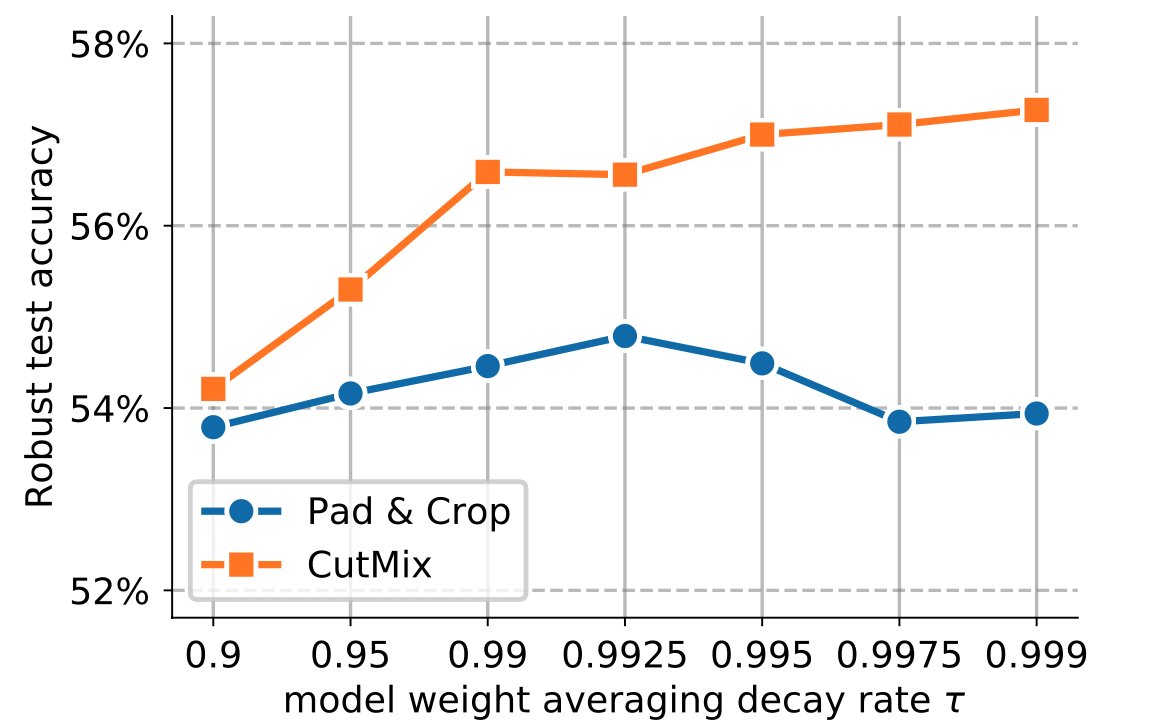
\includegraphics[width=0.7\linewidth]{pic/fig 8.png}
            \caption{Robust test accuracy against AA+MT with $\epsilon_\infty = 8/255$ on CIFAR-10 as we vary the decay rate of the model weight averaging. The model is a WRN-28-10, which is trained either with \textit{CutMix} or \textit{Pad \& Crop}.}
            \label{fig:fig8}
    \end{figure}
\end{frame}

\begin{frame}{Conclusion}
    \begin{itemize}[<+-| alert@+>] % stepwise alerts
        \item Contrary to previous works, which have tried data augmentation techniques to train adversarially robust models without success, we demonstrate that combining data augmentations with model weight averaging can significantly improve robustness.
        \item We also provide insights on why weight averaging works better with data augmentations which reduce robust overfitting.
        \item We show in fact that model snapshots of a same run have the same total robust accuracy but they greatly differ at the individual prediction level, thus allowing a performance boost when ensembling these snapshots.
    \end{itemize}
\end{frame}

\begin{frame}{Future Works}
    \begin{figure}
        \begin{minipage}{.45\textwidth}
            \centering
            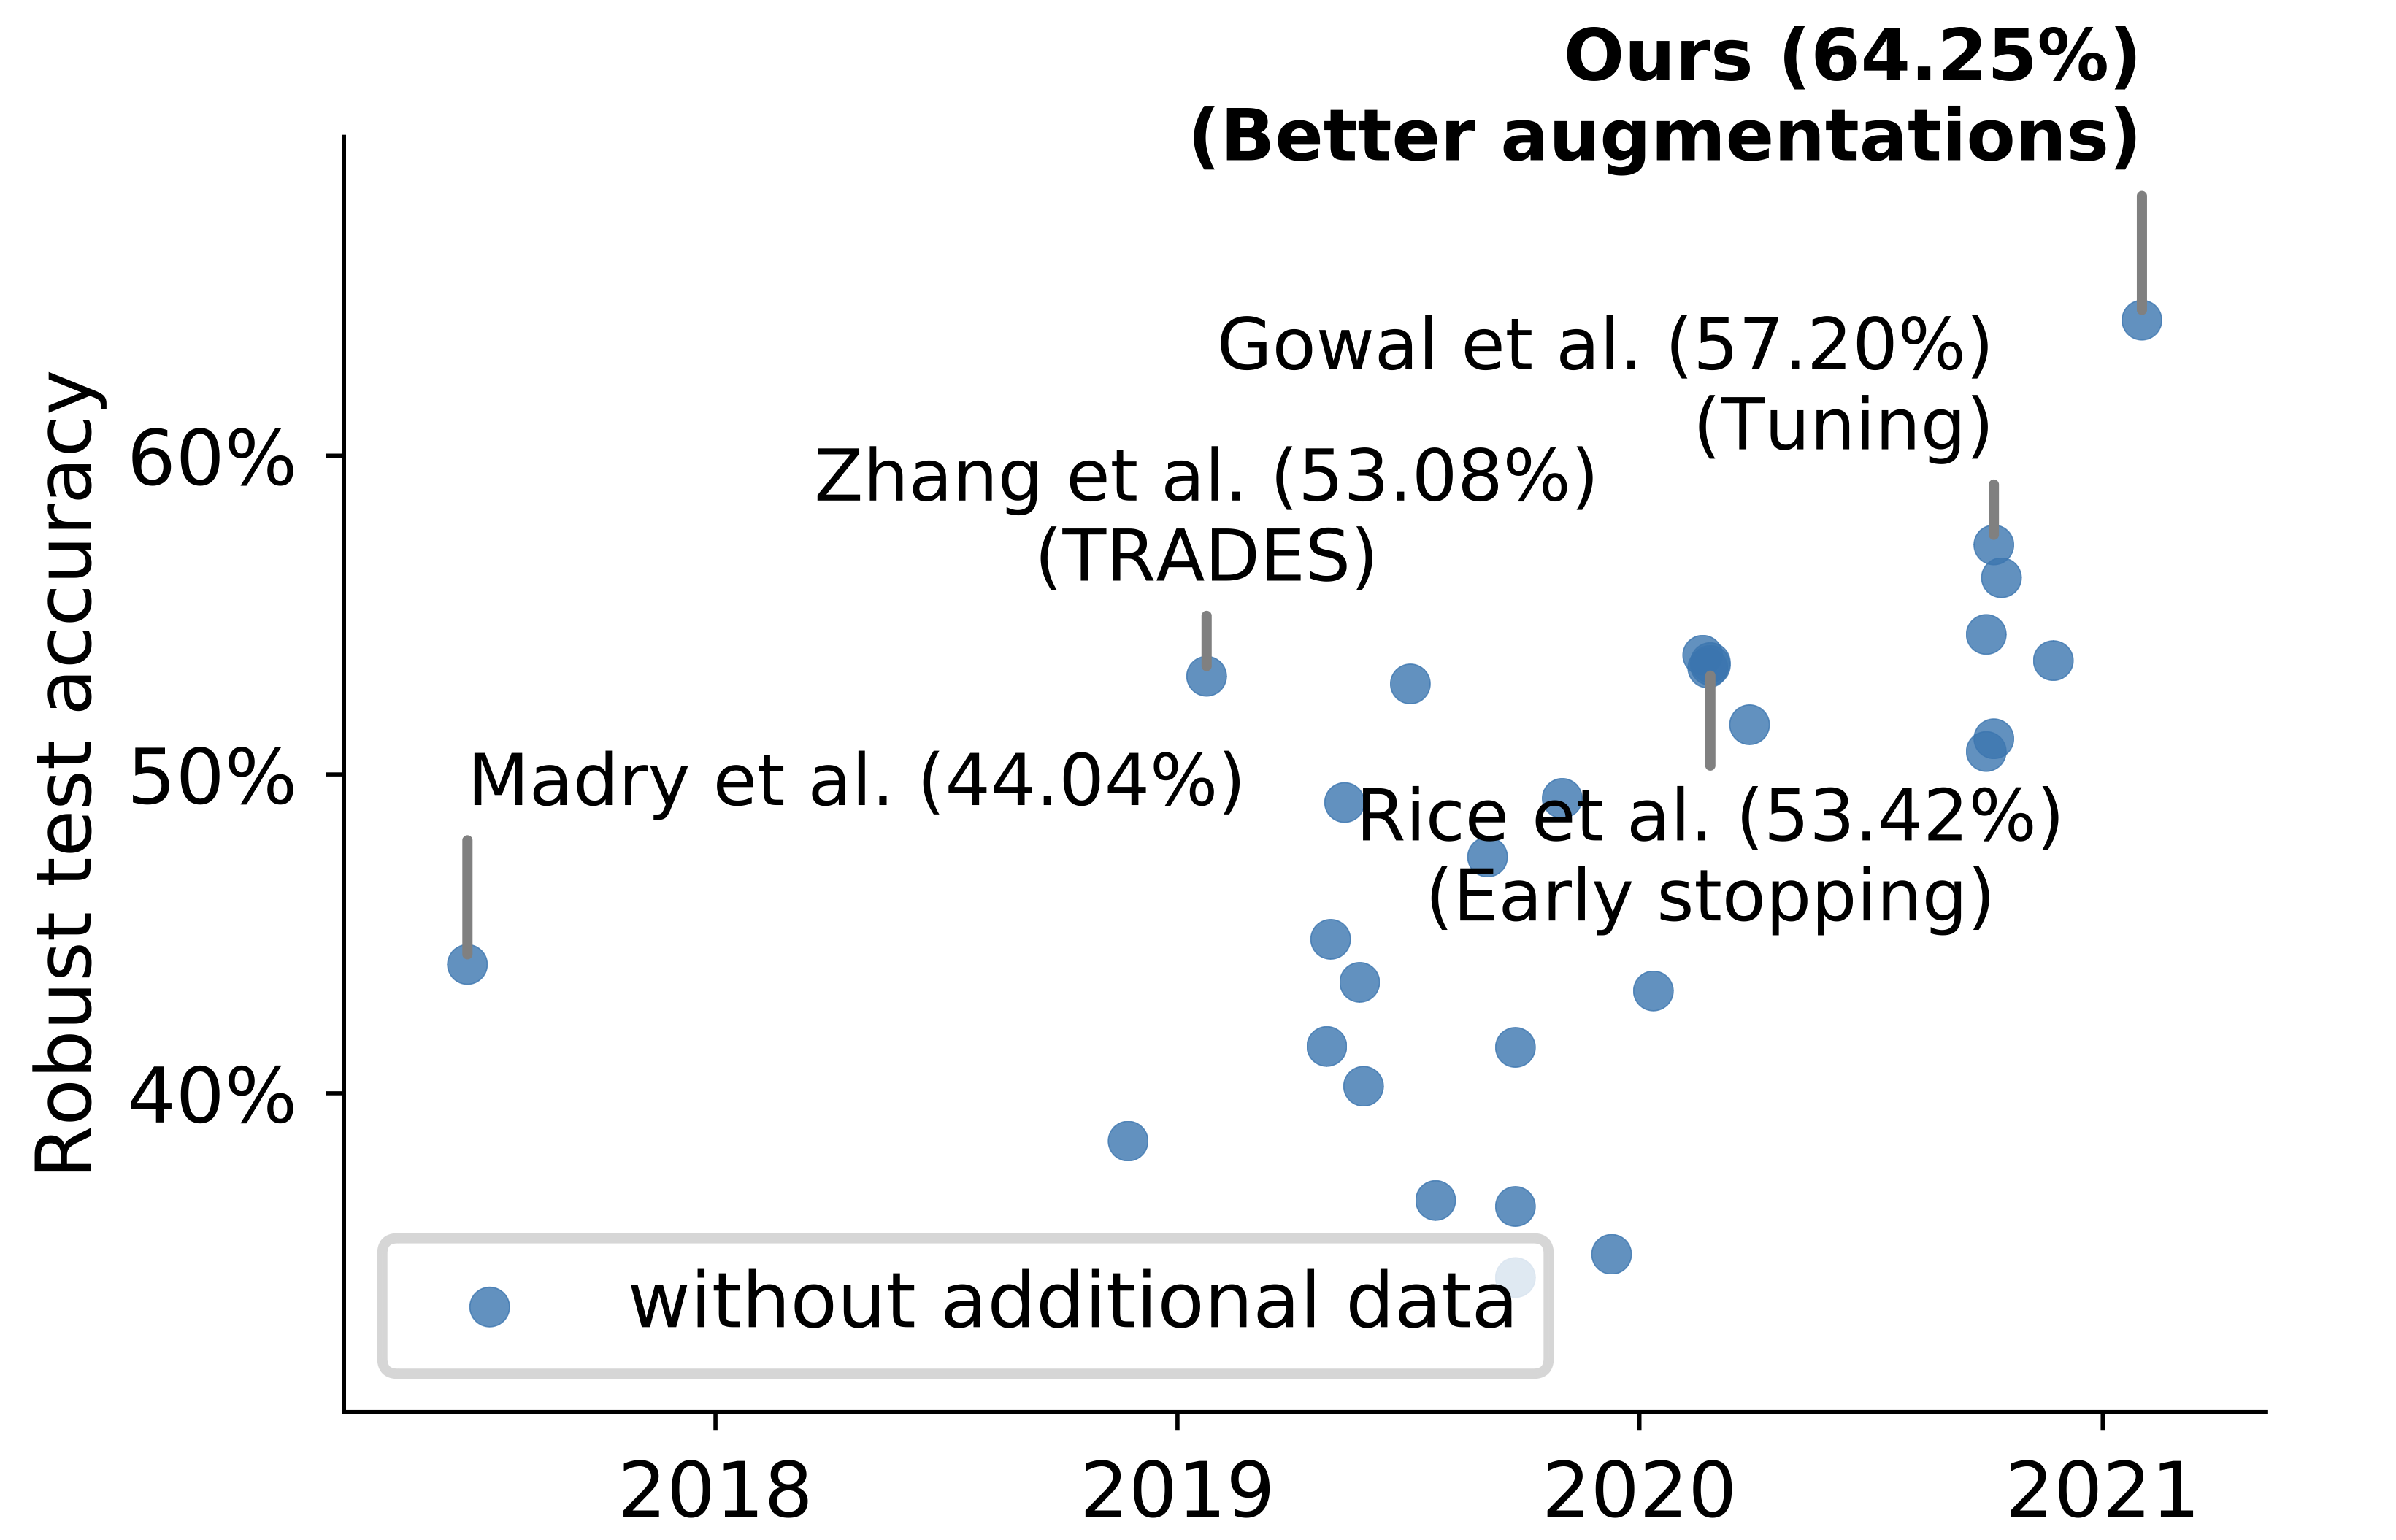
\includegraphics[width=\linewidth]{pic/oct 21.png}
            \caption{Fixing Data Augmentation to Improve Adversarial Robustness}
            \label{fig:oct21}
        \end{minipage}
        \begin{minipage}{.45\textwidth}
            \centering
            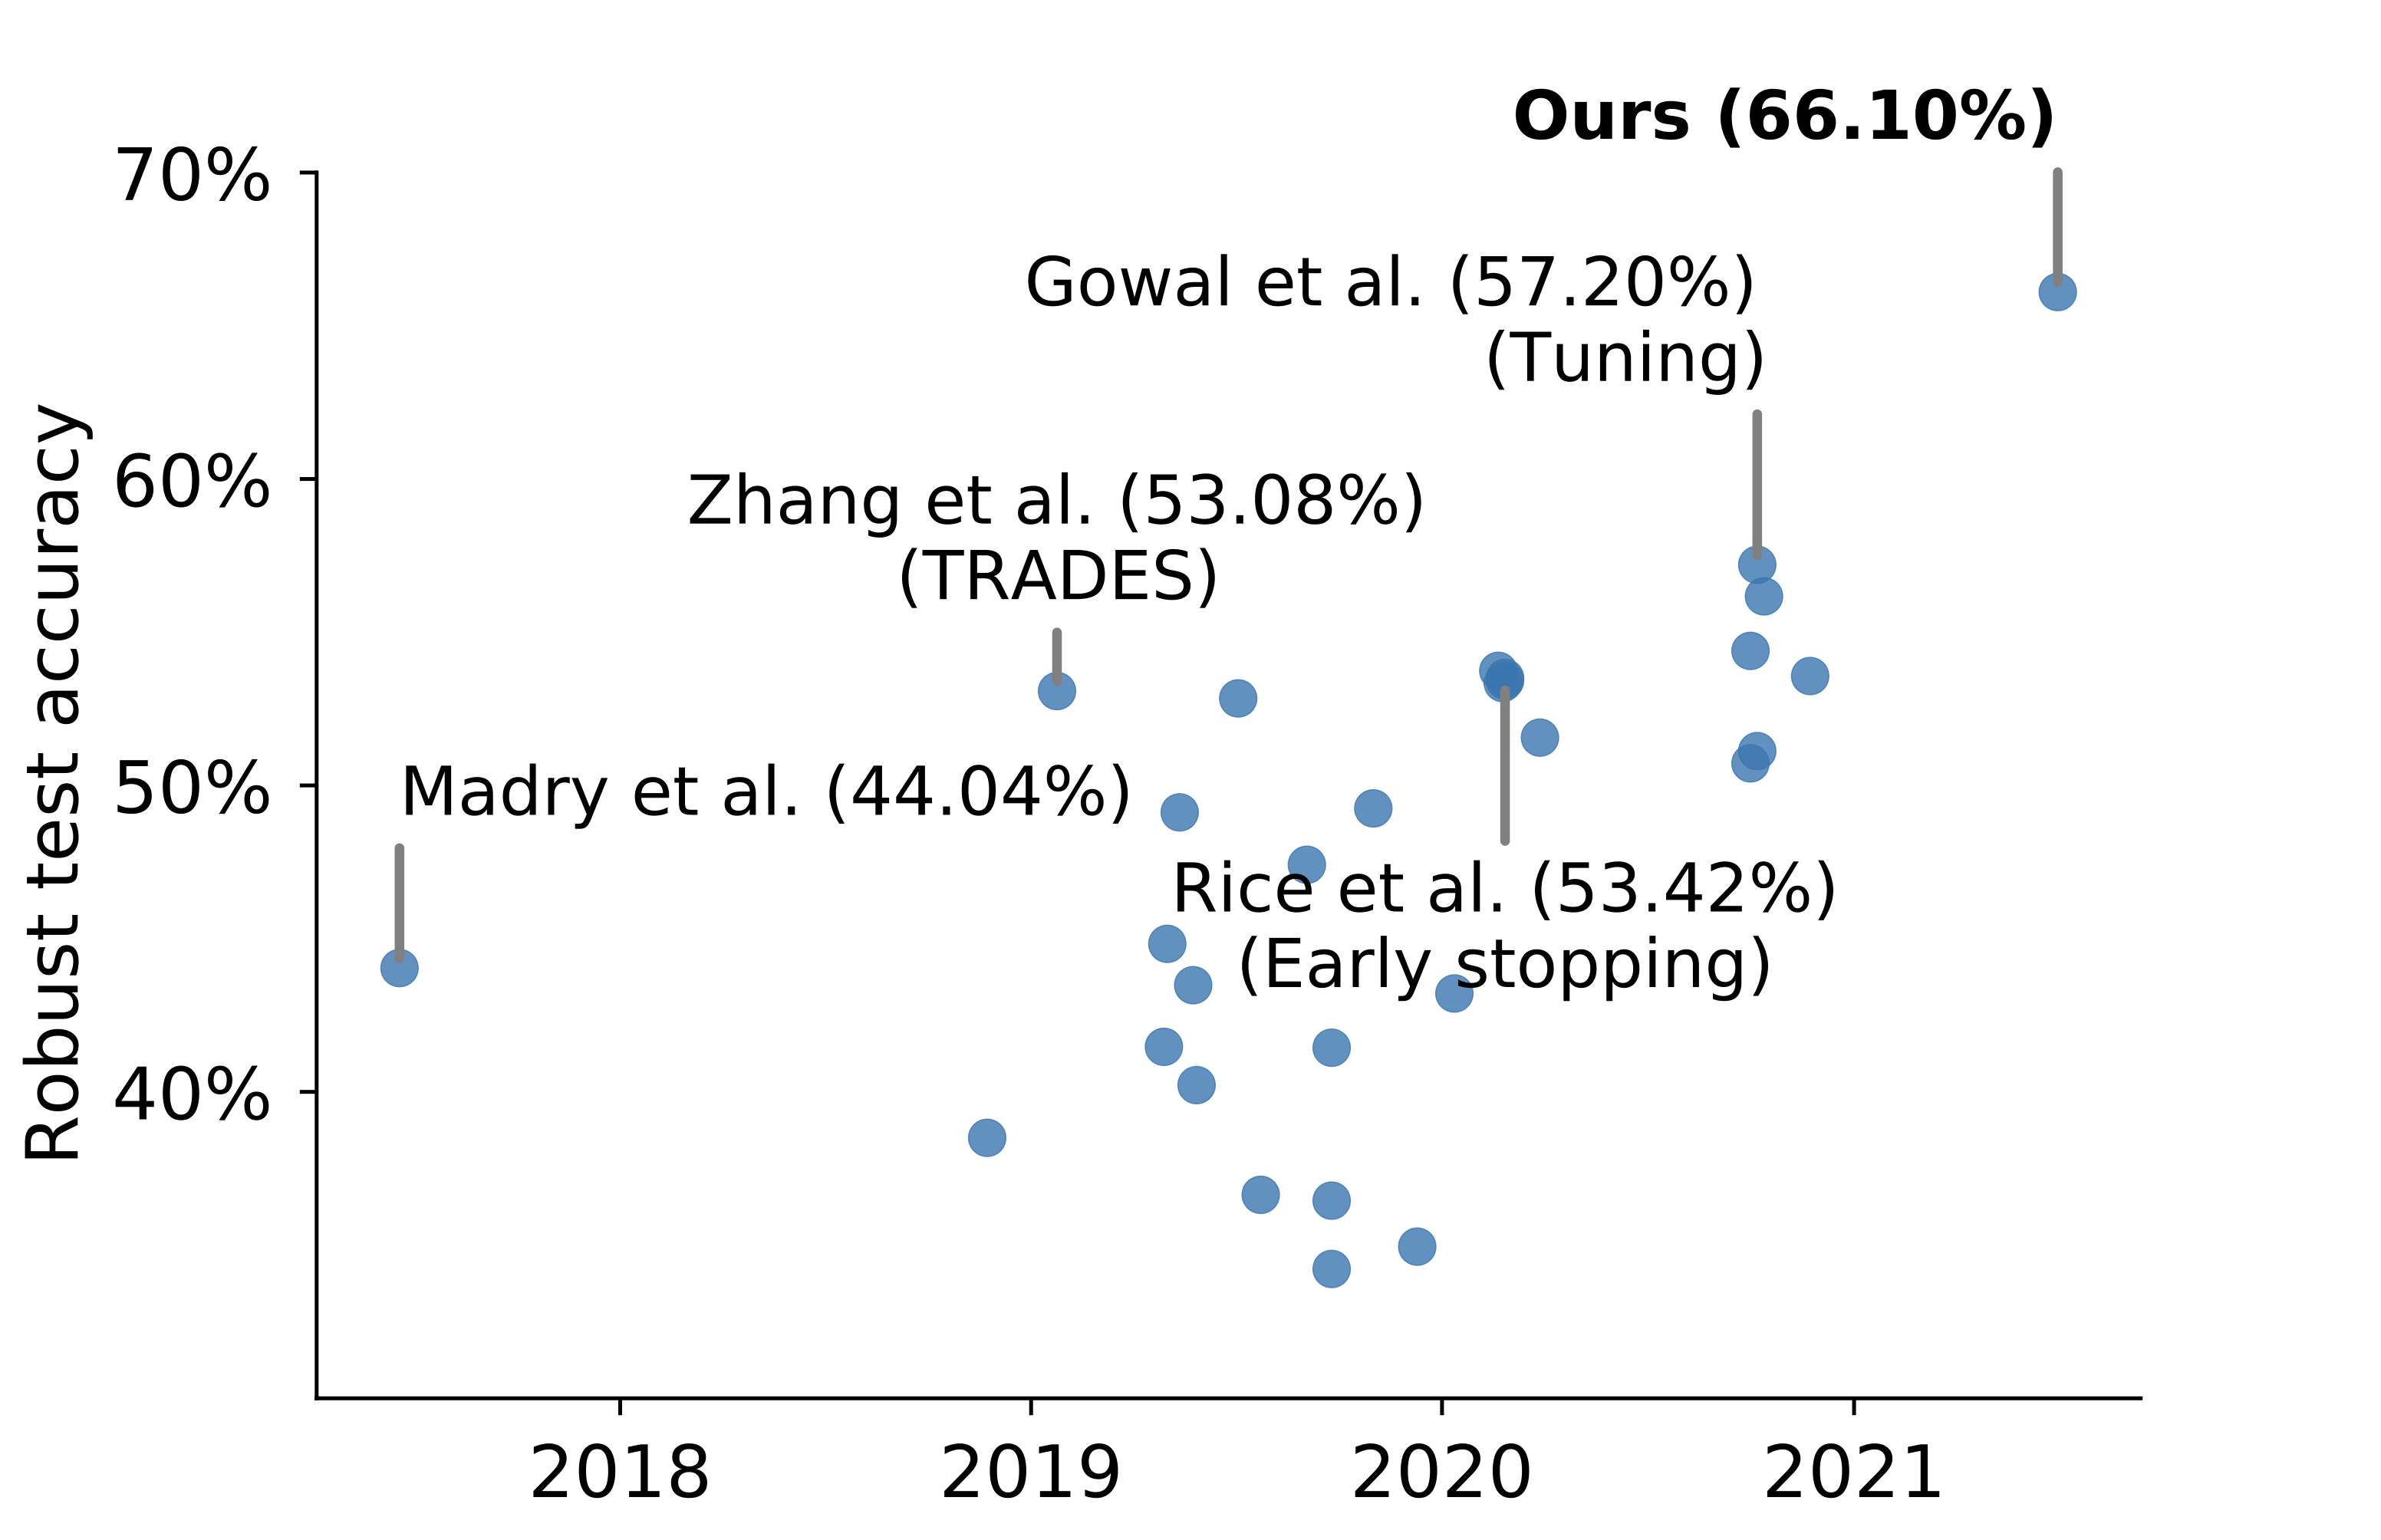
\includegraphics[width=\linewidth]{pic/dec 21.png}
            \caption{Improving Robustness using Generated Data}
            \label{fig:dec21}
        \end{minipage}
    \end{figure}
    
\end{frame}

\begin{frame}{Refrences}
    \bibliography{ref}
    \bibliographystyle{ieeetr}
    \nocite{*}
\end{frame}

% \begin{frame}
%     \begin{center}
%         {\Huge\calligra Thank You}
%     \end{center}
% \end{frame}

\end{document}